\section{Presentation Logic Layer}

%What pages will be present in your project? briefly indicate how your web site will be organized

The web application is divided in the following pages:
\begin{itemize}
    \item Homepage: HomePage of the webApp
    \item LoginPage: Page in which a user can login by providing his/her own credentials.
    \item UserPage: After a successful login, it’s possible to enter into the personal area which contains all the user data.
    \item Stats Page: An overview of users statistics that includes Body Measures, Goals, Diet and Exercise.
    \item Social Network Page: A simple social network page where the user can see other users post, like or comment those posts or publish his own post.
    \item Diet Page: An overview of user's diets which can be modified if int he 24h range simply create a new one
    \item Meal Page: It's possible to see an overview of the meals consumed by users in various days. The user can register a meal through the button.
    \item Exercise Page: An overview of the user's exercises which can be modified by the user or he can add a new one.
\end{itemize}

\subsection{Pages mockup}

%For the main pages put a mockup and describe it in detail.
\begin{center}
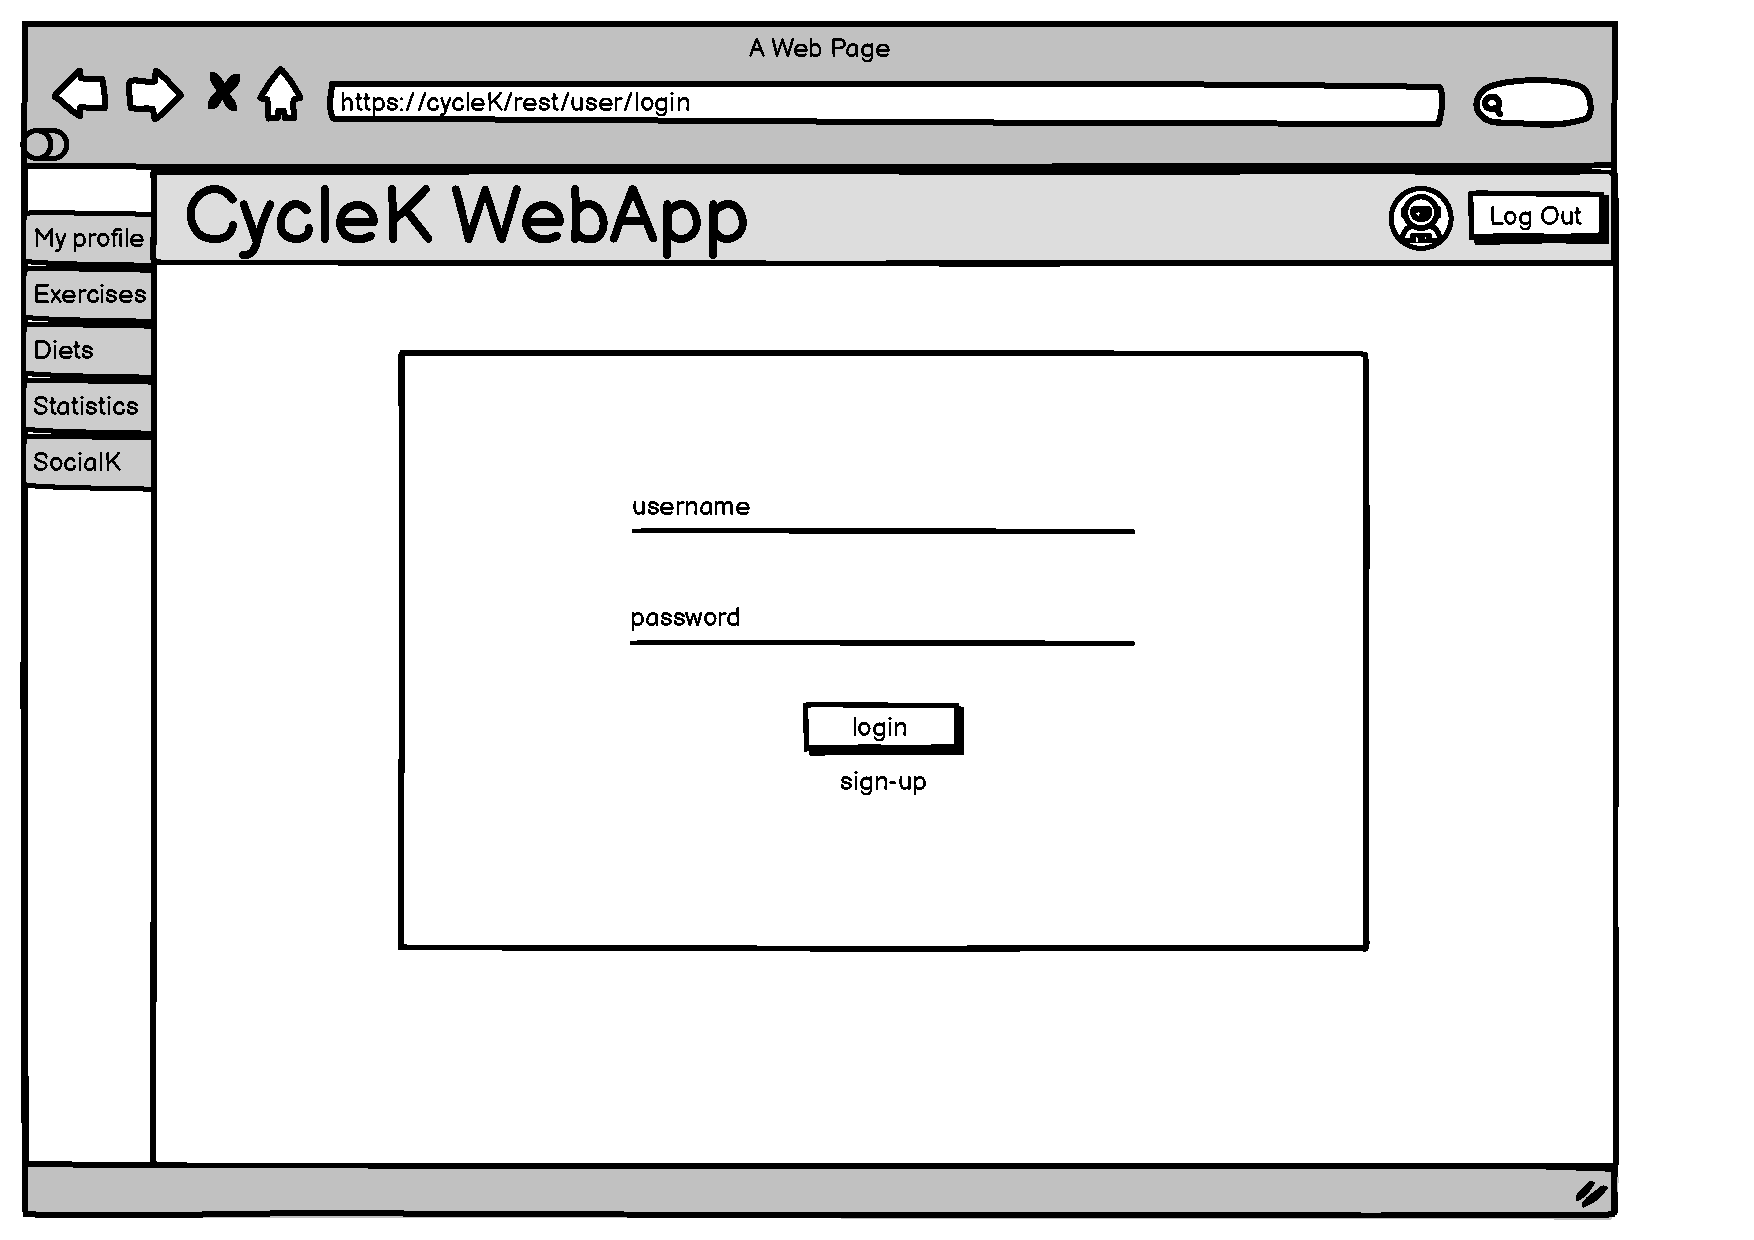
\includegraphics[scale=0.47]{Resources/Mockup/LoginPage.pdf}\\
Login Page
\end{center}

\begin{center}
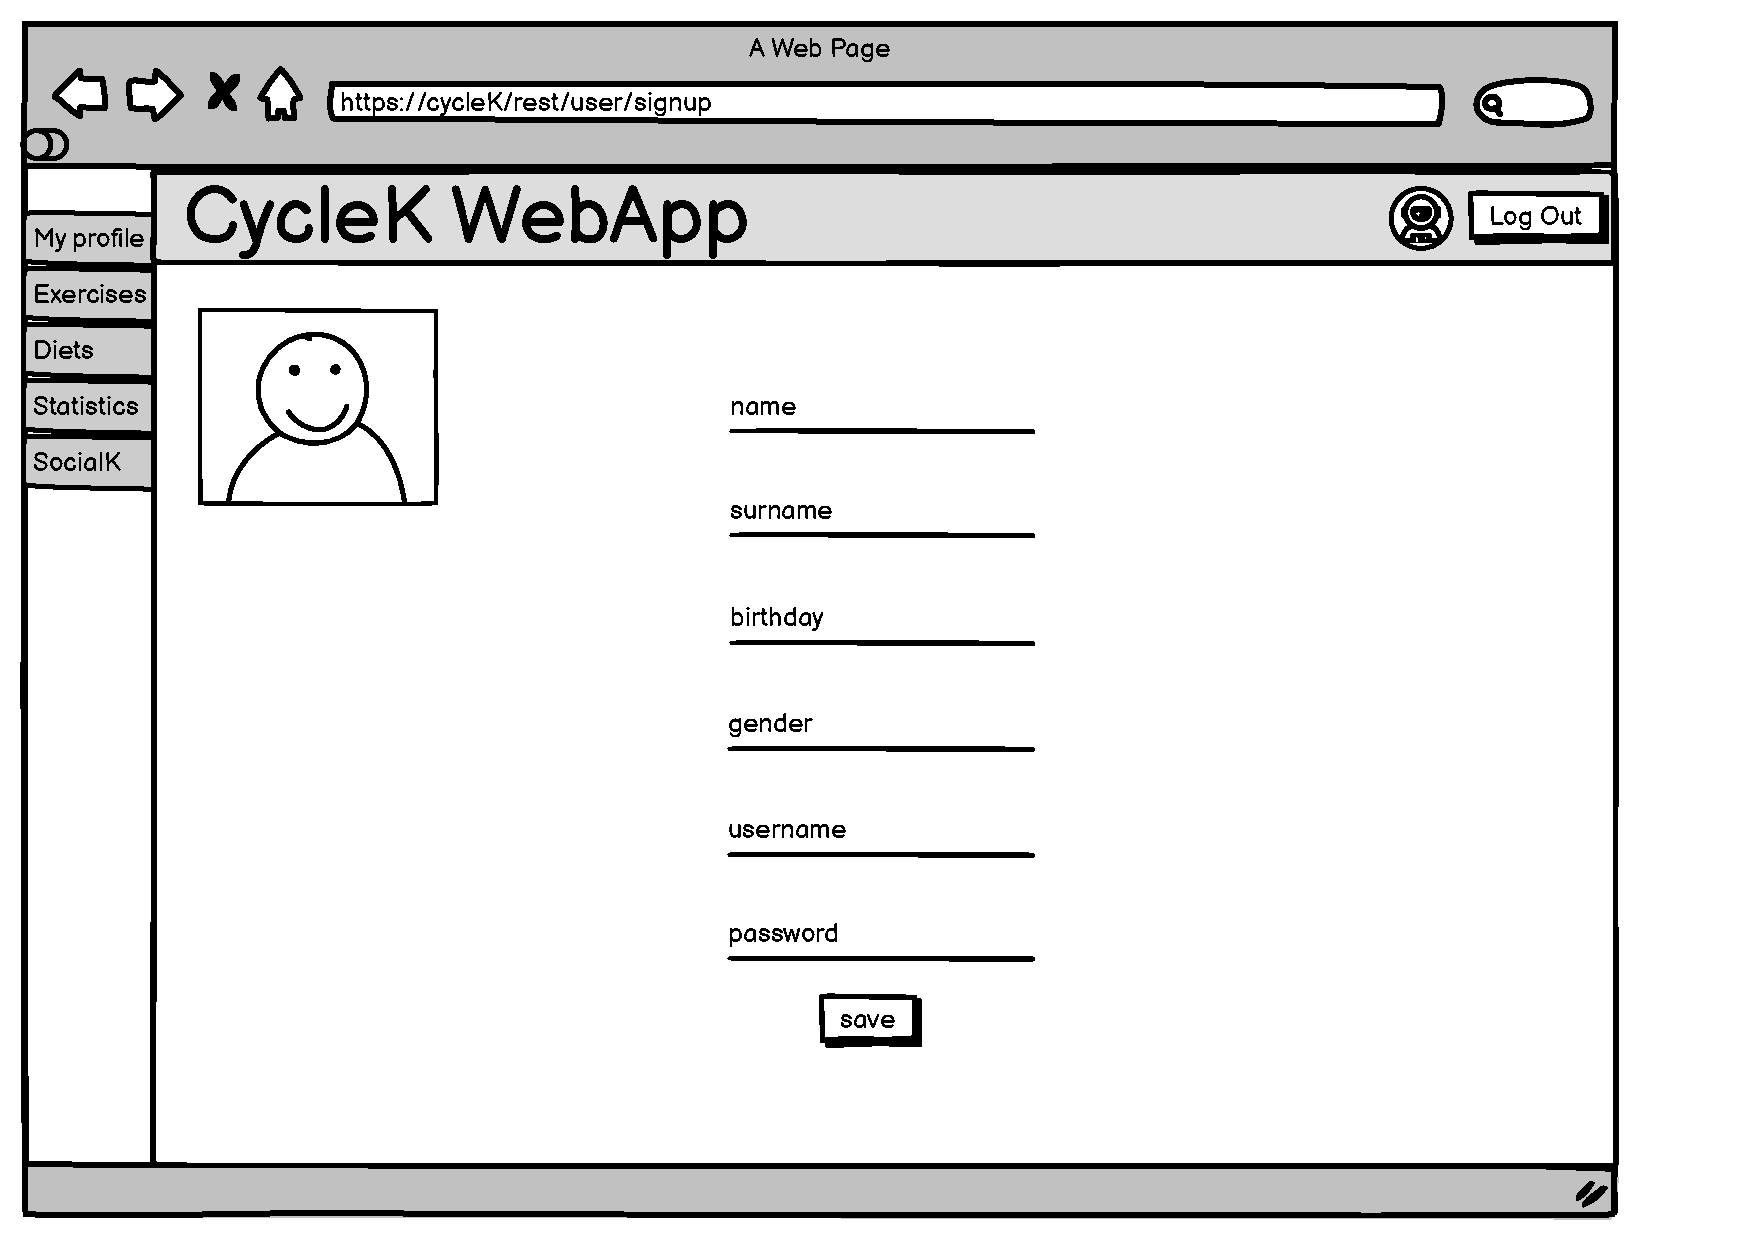
\includegraphics[scale=0.47]{Resources/Mockup/UserPage.pdf}\\
User Profile Page
\end{center}

% excercise
\begin{center}
\includegraphics[scale=0.47]{Resources/Mockup/Exercises.pdf}\\
Exercise Page
\end{center}

\begin{center}
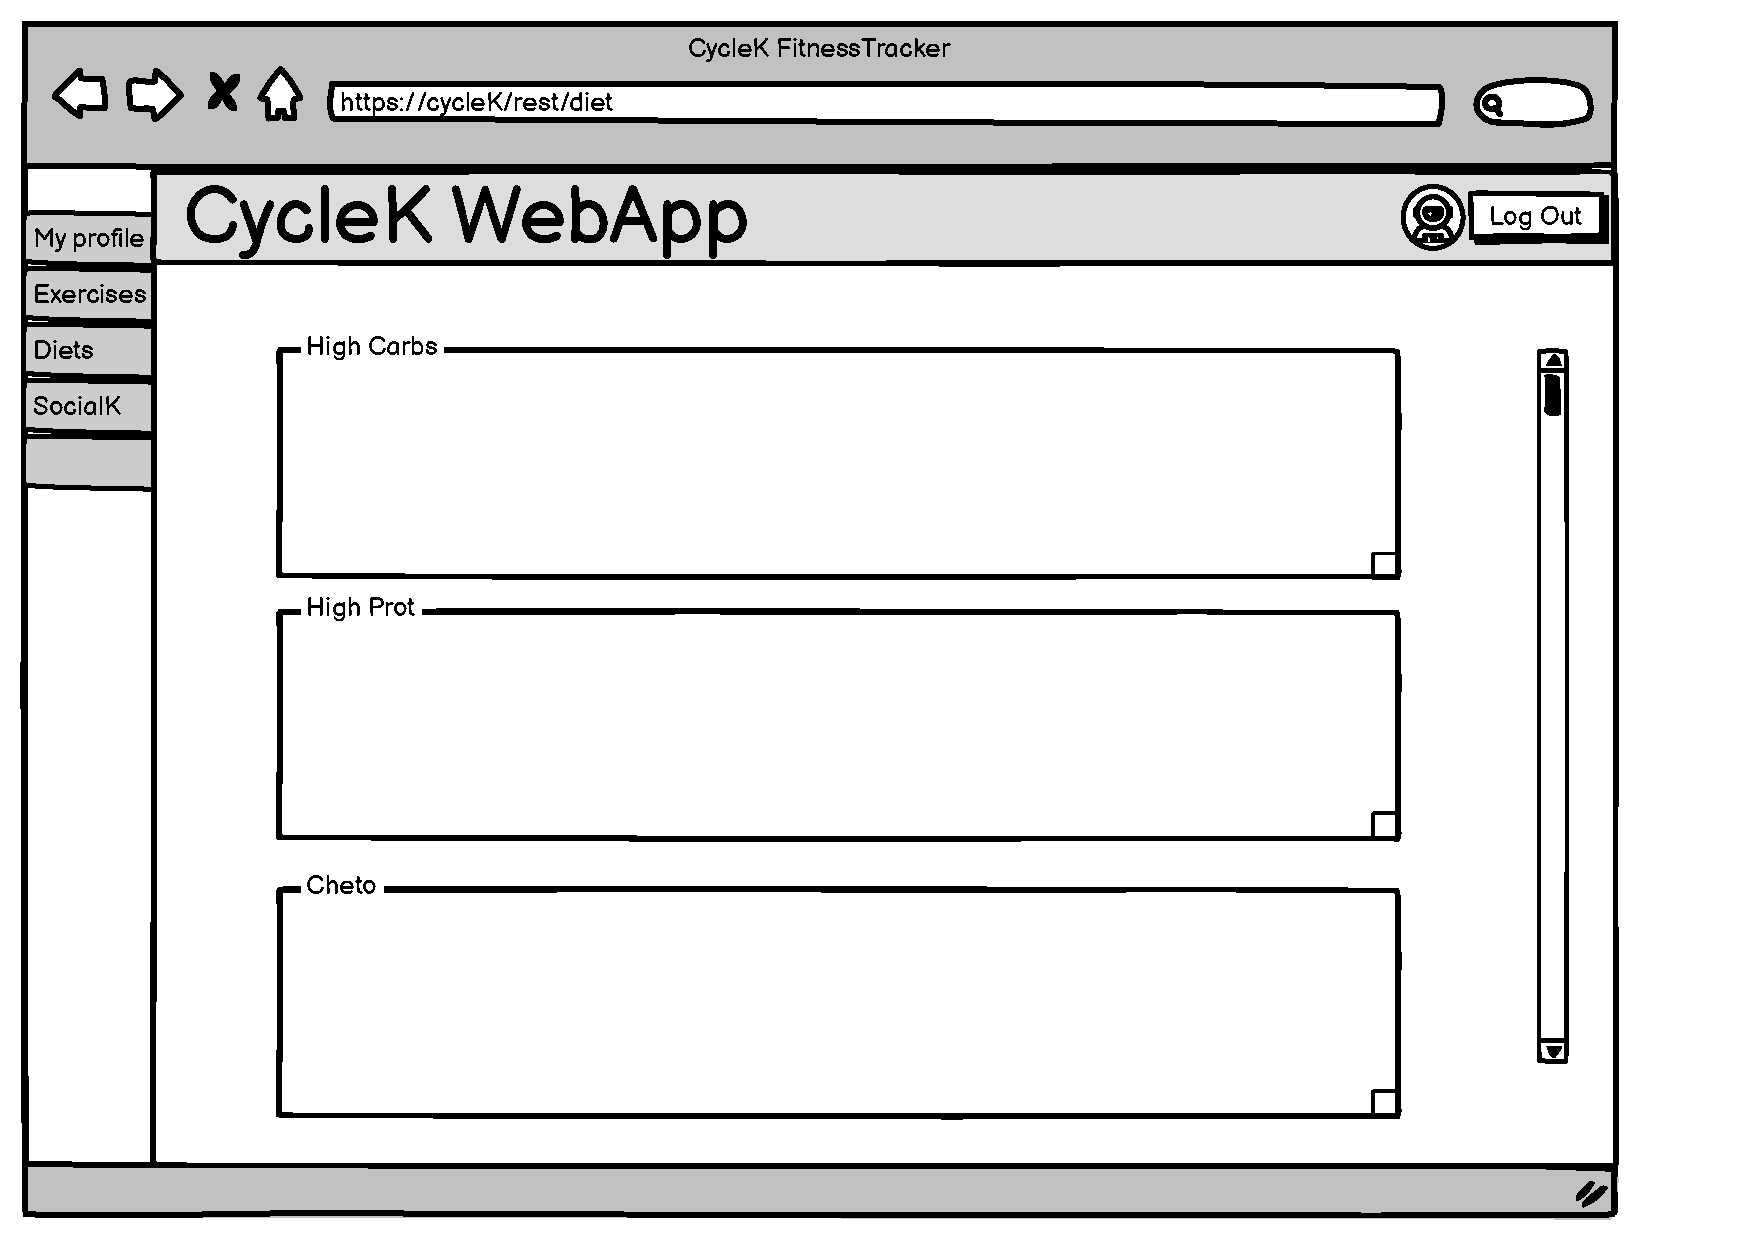
\includegraphics[scale=0.47]{Resources/Mockup/DietMockup.pdf}\\
Diet Page
\end{center}
% meal
\begin{center}
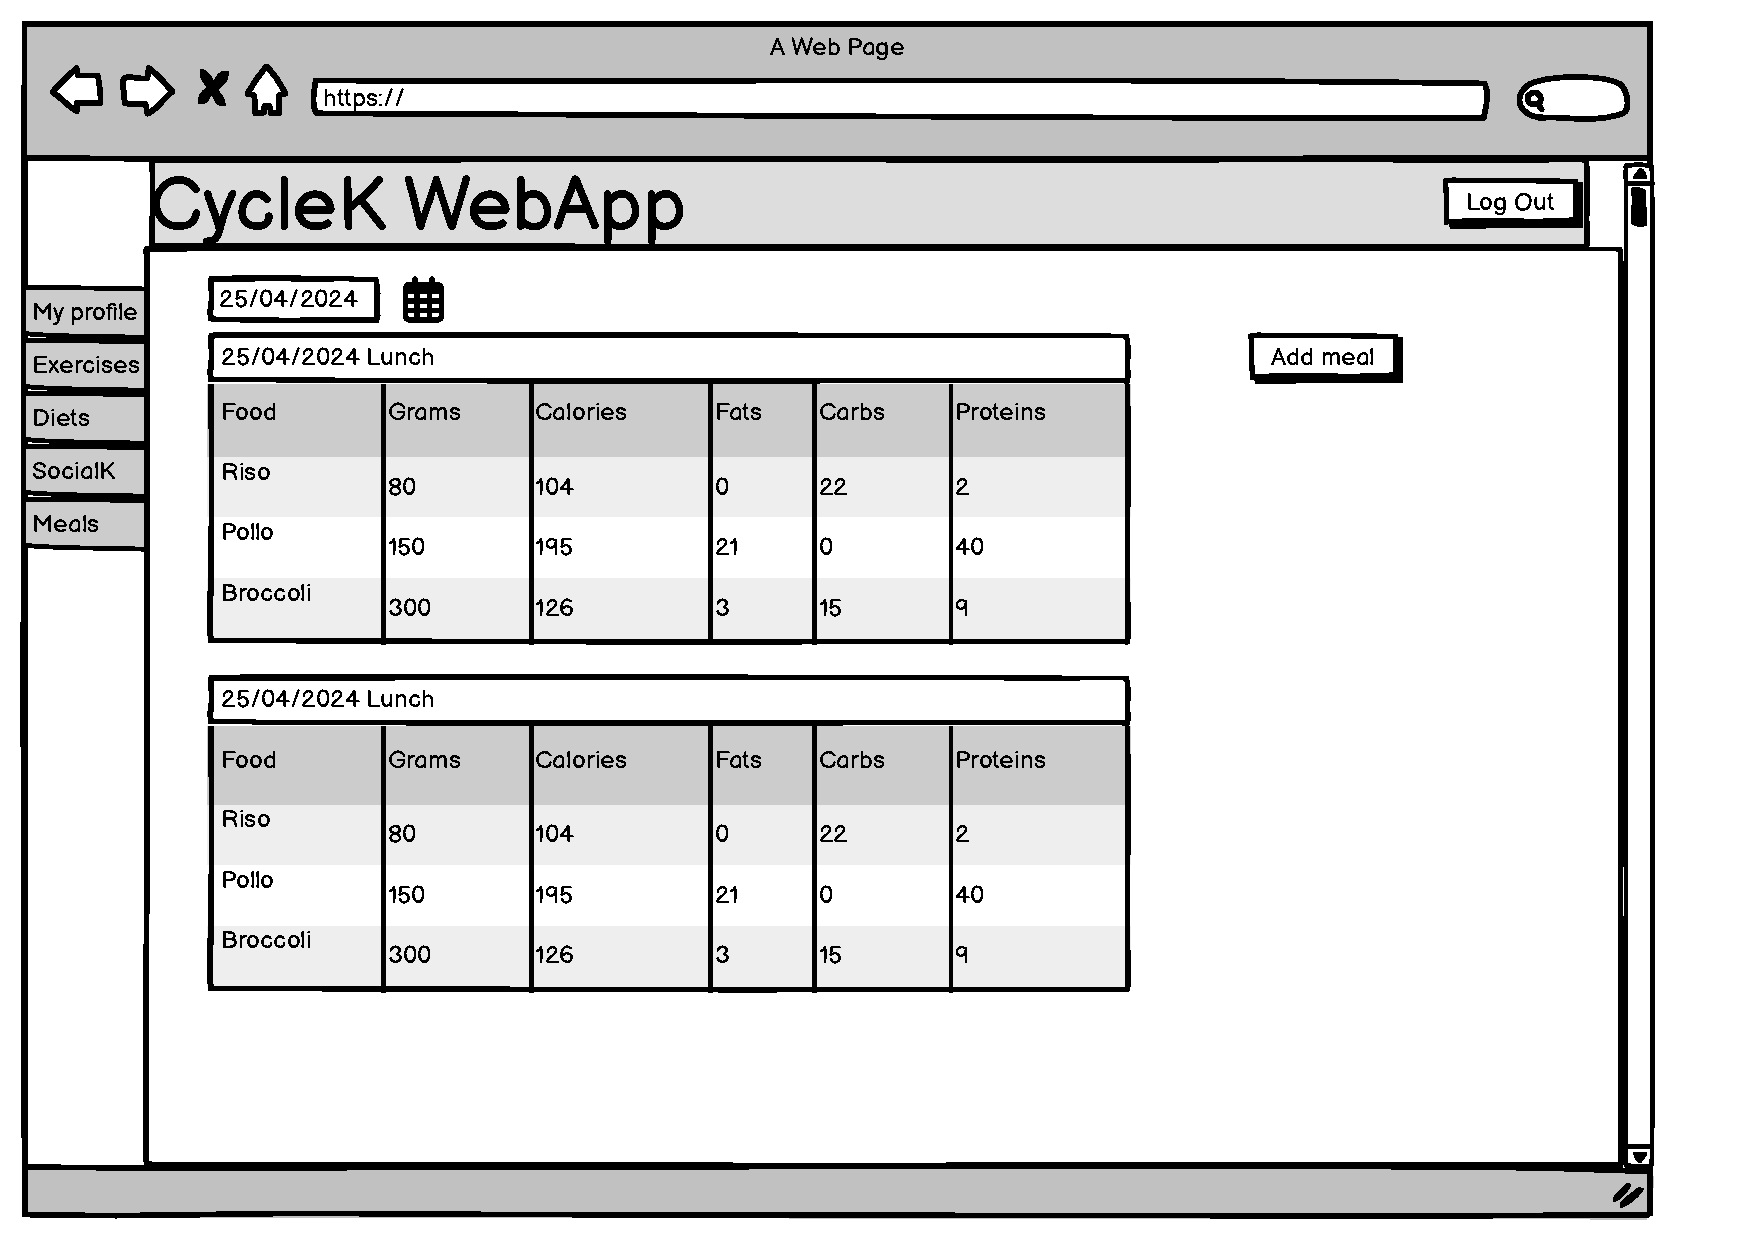
\includegraphics[scale=0.47]{Resources/Mockup/Meals.pdf}\\
Meals Page
\end{center}

\begin{center}
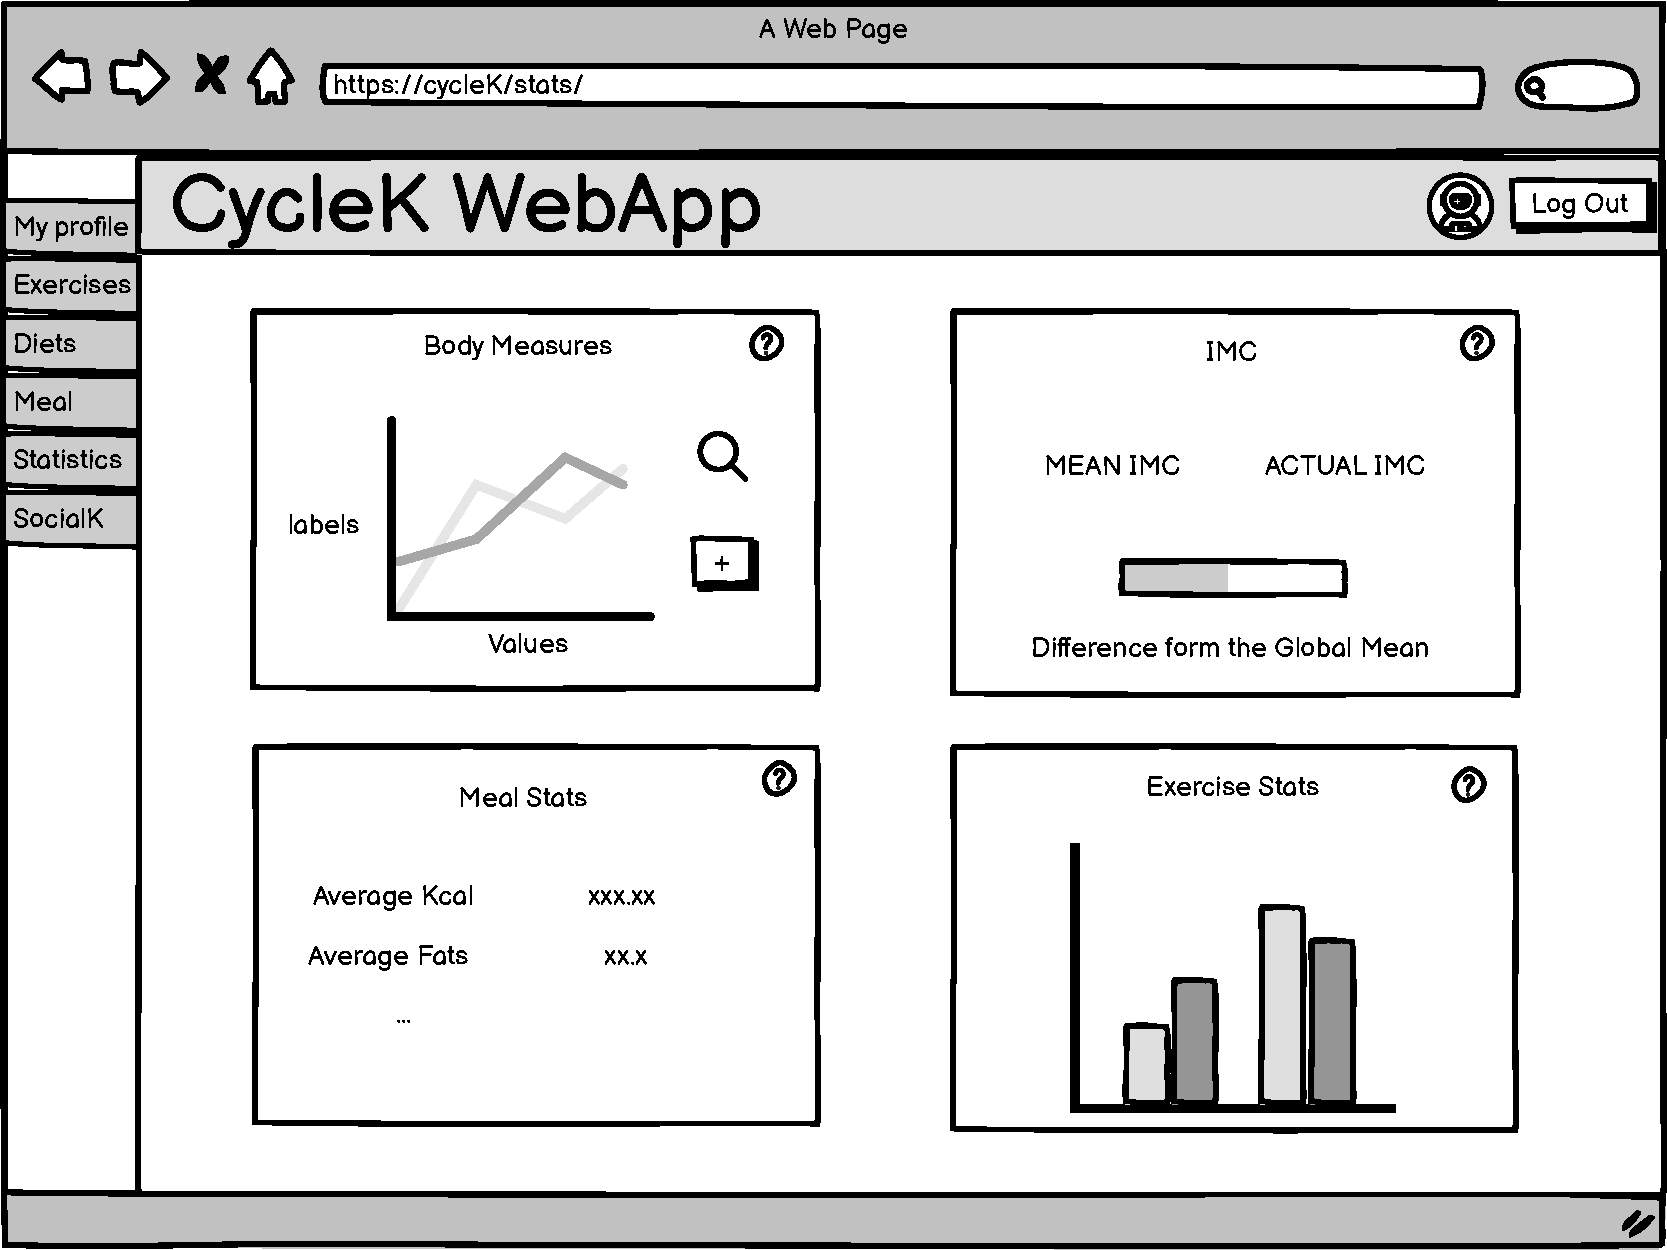
\includegraphics[scale=0.47]{Resources/Mockup/Stats.pdf}\\
Stats Page
\end{center}
In this Page the user have a general overview of its progress in all fields. A chart will show a comparison among all measures the user inserted with the apposite button, this chart allows the tracking of gain and loos in weight, fatty and lean mass. Another Chart will show the User current and mean IMC computed with its measures and the metrics is compared with the global mean IMC, this allows the user to know his place with respect to other people that are using our app.
Other two charts will show some data obtained from the user's meals and exercise to show the average food metrics intake like proteins and other and some exercise metrics. This charts should help the user to understand whether they are flexible or not about diet and exercise.

\begin{center}
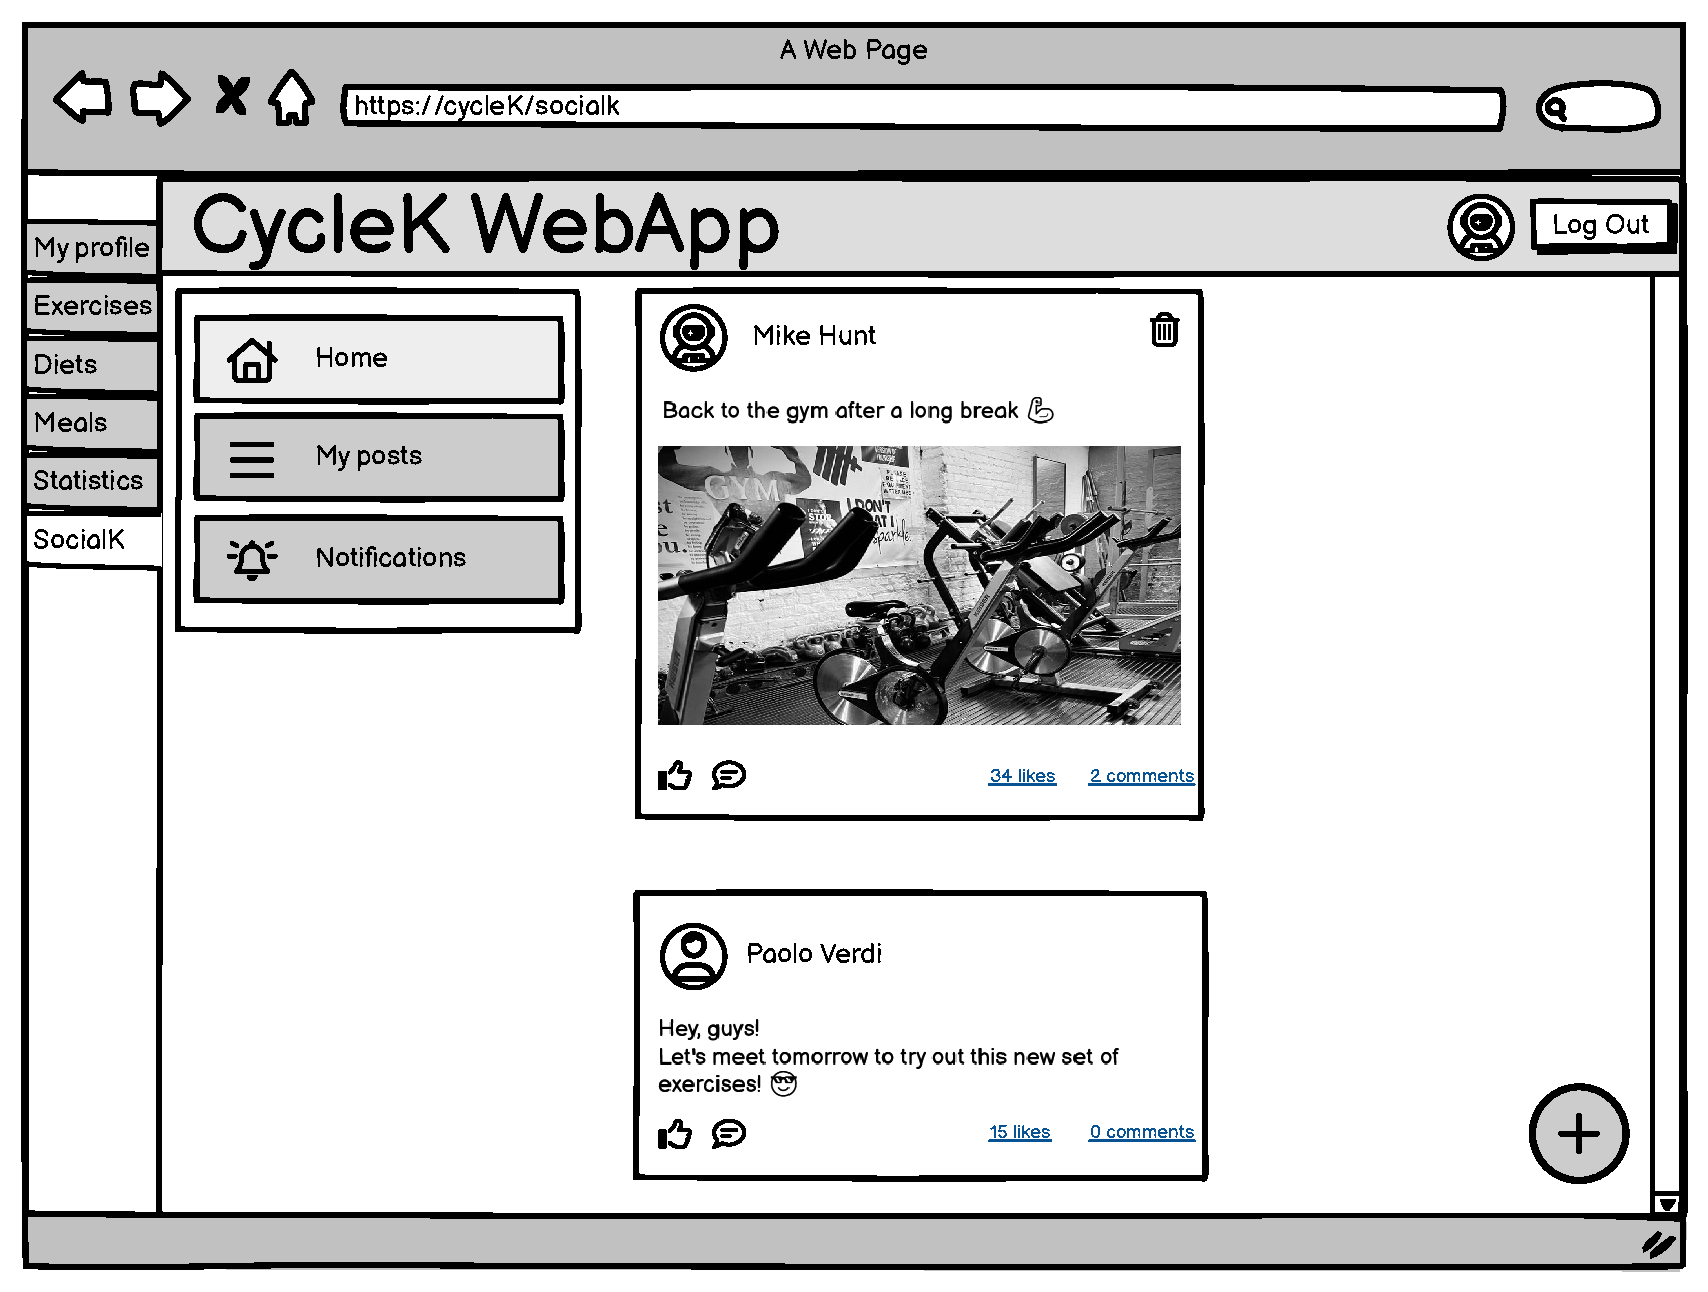
\includegraphics[scale=0.47]{Resources/Mockup/socialk_home.pdf}\\
SocialK home page
\end{center}

\begin{center}
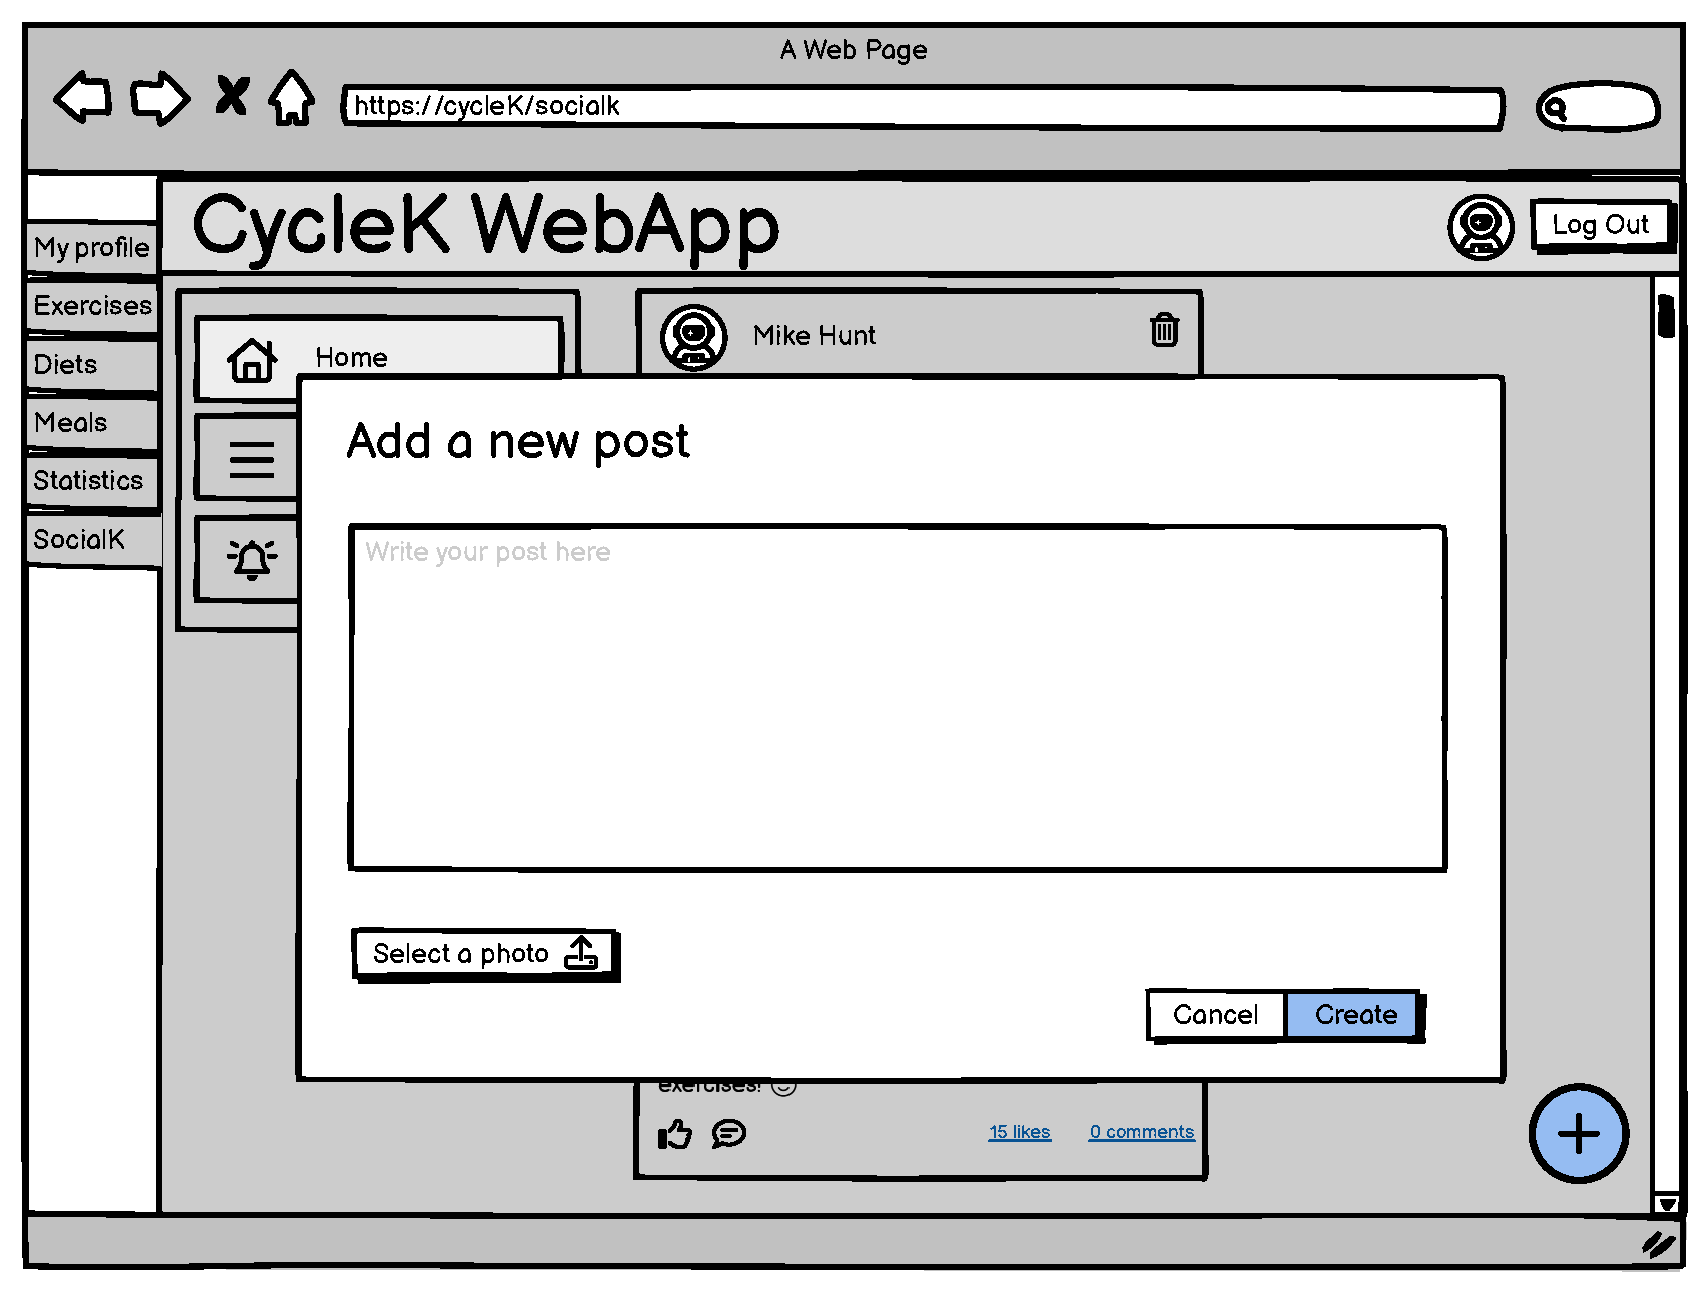
\includegraphics[scale=0.47]{Resources/Mockup/socialk_post.pdf}\\
Creation of a new post
\end{center}

\begin{center}
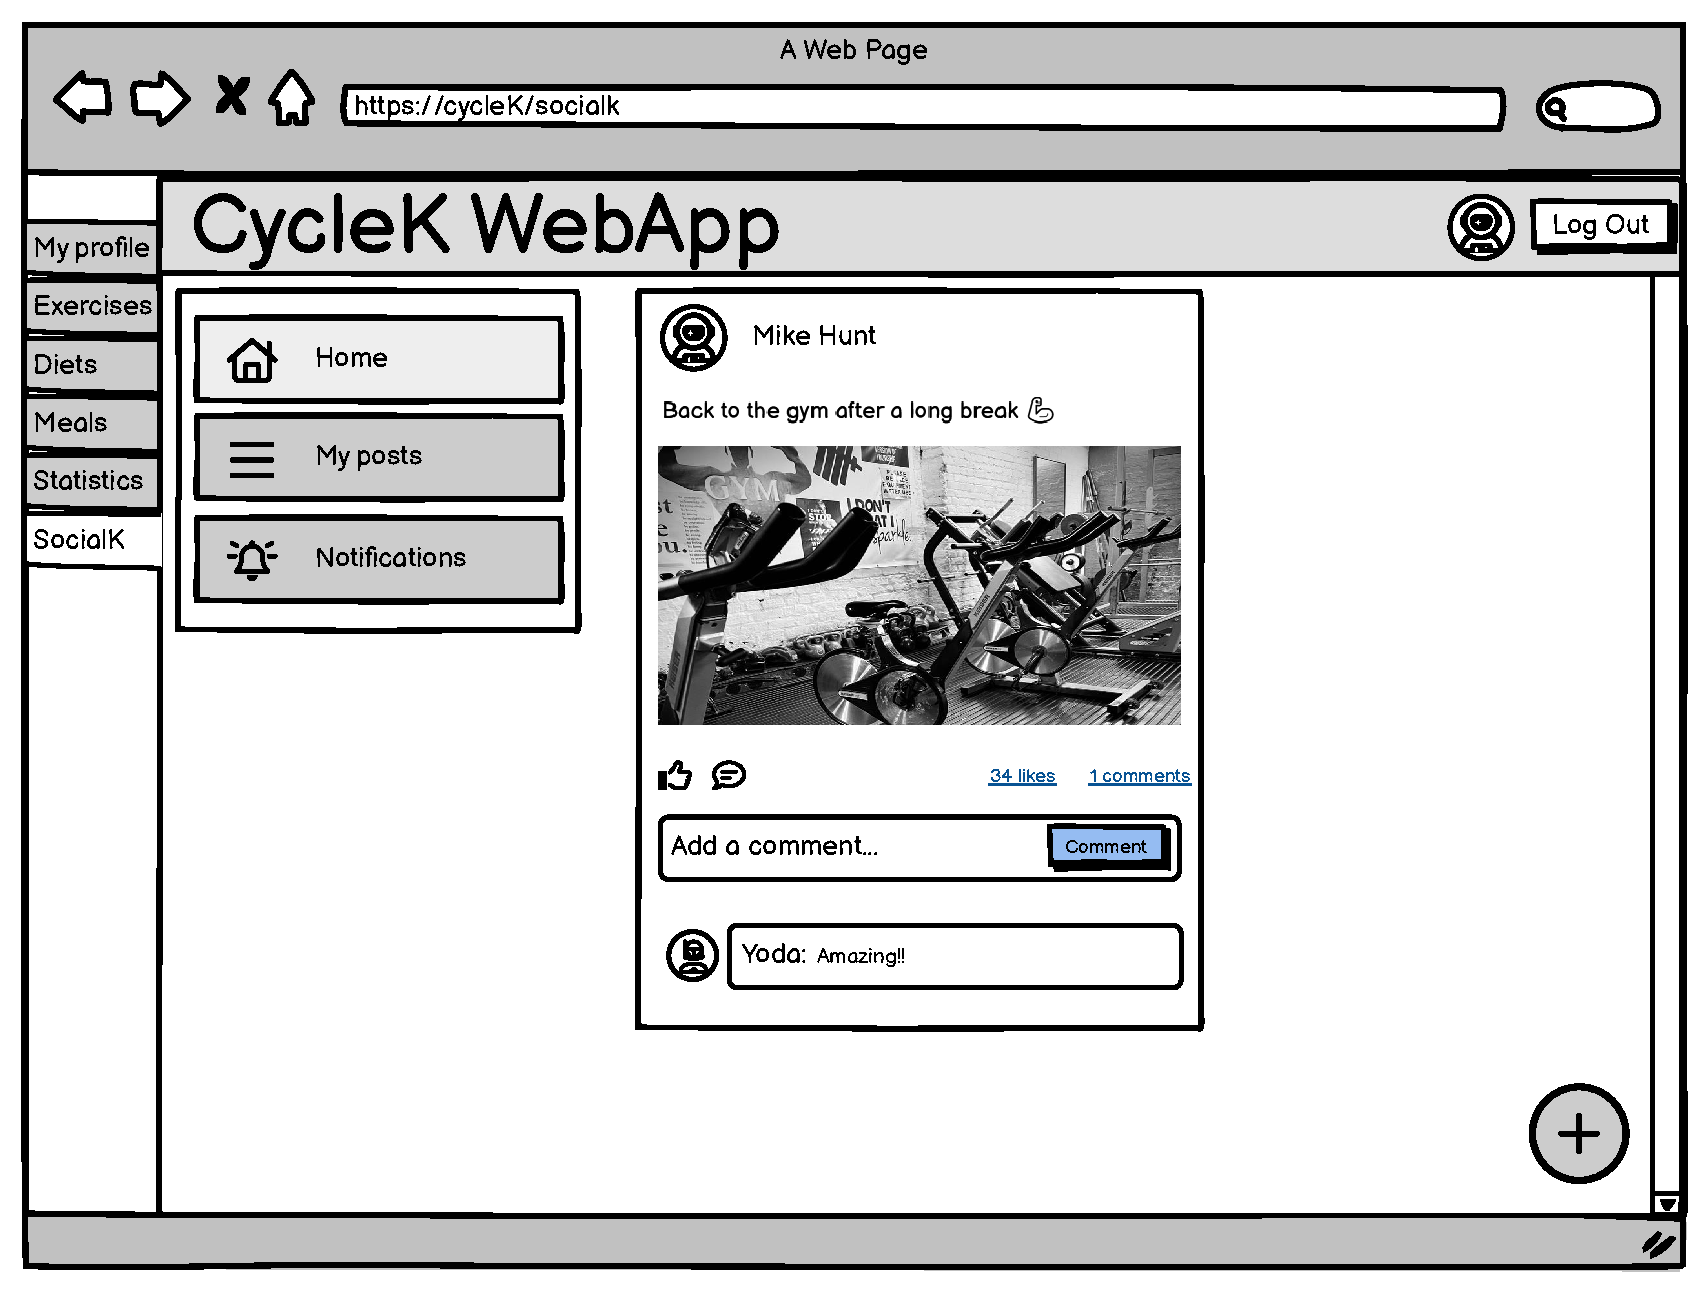
\includegraphics[scale=0.47]{Resources/Mockup/socialk_comment.pdf}\\
Creation of a new comment
\end{center}

